\documentclass{standalone}

\usepackage{graphicx}
\usepackage{tikz}
\usetikzlibrary{arrows}
\usetikzlibrary{decorations.markings}

\definecolor{purple}{RGB}{99,0,129}
\definecolor{gold}{RGB}{255,204,26}

\pgfdeclarelayer{bg}    % declare background layer
\pgfsetlayers{bg,main}  % set the order of the layers (main is the standard layer)

\begin{document}

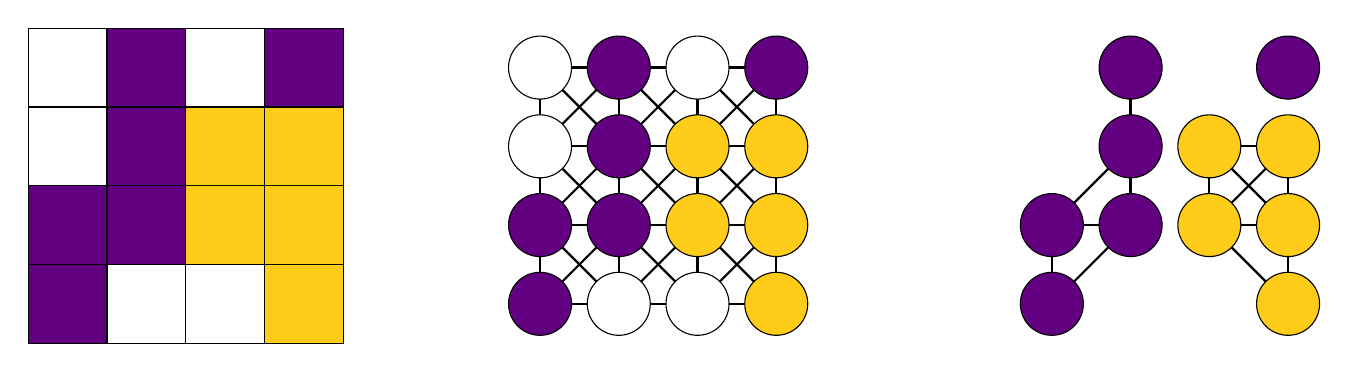
\begin{tikzpicture}
  \draw[fill=purple] (0, 0) rectangle (1, 1);
  \draw[fill=white] (1, 0) rectangle (2, 1);
  \draw[fill=white] (2, 0) rectangle (3, 1);
  \draw[fill=gold] (3, 0) rectangle (4, 1);
  \draw[fill=purple] (0, 1) rectangle (1, 2);
  \draw[fill=purple] (1, 1) rectangle (2, 2);
  \draw[fill=gold] (2, 1) rectangle (3, 2);
  \draw[fill=gold] (3, 1) rectangle (4, 2);
  \draw[fill=white] (0, 2) rectangle (1, 3);
  \draw[fill=purple] (1, 2) rectangle (2, 3);
  \draw[fill=gold] (2, 2) rectangle (3, 3);
  \draw[fill=gold] (3, 2) rectangle (4, 3);
  \draw[fill=white] (0, 3) rectangle (1, 4);
  \draw[fill=purple] (1, 3) rectangle (2, 4);
  \draw[fill=white] (2, 3) rectangle (3, 4);
  \draw[fill=purple] (3, 3) rectangle (4, 4);

  \draw[fill=white] (6.5, 2.5) circle (0.4) node (w1) {};
  \draw[fill=white] (6.5, 3.5) circle (0.4) node (w2) {};
  \draw[fill=white] (7.5, 0.5) circle (0.4) node (w3) {};
  \draw[fill=white] (8.5, 0.5) circle (0.4) node (w4) {};
  \draw[fill=white] (8.5, 3.5) circle (0.4) node (w5) {};
  \draw[fill=purple] (6.5, 0.5) circle (0.4) node (p11) {};
  \draw[fill=purple] (6.5, 1.5) circle (0.4) node (p21) {};
  \draw[fill=purple] (7.5, 1.5) circle (0.4) node (p31) {};
  \draw[fill=purple] (7.5, 2.5) circle (0.4) node (p41) {};
  \draw[fill=purple] (7.5, 3.5) circle (0.4) node (p51) {};
  \draw[fill=purple] (9.5, 3.5) circle (0.4) node (p61) {};
  \draw[fill=gold] (9.5, 0.5) circle (0.4) node (g11) {};
  \draw[fill=gold] (8.5, 1.5) circle (0.4) node (g21) {};
  \draw[fill=gold] (9.5, 1.5) circle (0.4) node (g31) {};
  \draw[fill=gold] (8.5, 2.5) circle (0.4) node (g41) {};
  \draw[fill=gold] (9.5, 2.5) circle (0.4) node (g51) {};

  \begin{pgfonlayer}{bg}    % select the background layer
    \draw[thick] (w1) -- (w2);
    \draw[thick] (w1) -- (p21);
    \draw[thick] (w1) -- (p31);
    \draw[thick] (w1) -- (p41);
    \draw[thick] (w1) -- (p51);
    \draw[thick] (w2) -- (p41);
    \draw[thick] (w2) -- (p51);
    \draw[thick] (w3) -- (p11);
    \draw[thick] (w3) -- (p21);
    \draw[thick] (w3) -- (p31);
    \draw[thick] (w3) -- (g21);
    \draw[thick] (w4) -- (w3);
    \draw[thick] (w4) -- (p31);
    \draw[thick] (w4) -- (g21);
    \draw[thick] (w4) -- (g31);
    \draw[thick] (w4) -- (g11);
    \draw[thick] (w5) -- (p51);
    \draw[thick] (w5) -- (p61);
    \draw[thick] (w5) -- (p41);
    \draw[thick] (w5) -- (g41);
    \draw[thick] (w5) -- (g51);
    \draw[thick] (p11) -- (p21);
    \draw[thick] (p11) -- (p31);
    \draw[thick] (p21) -- (p31);
    \draw[thick] (p21) -- (p41);
    \draw[thick] (p31) -- (p41);
    \draw[thick] (p41) -- (p51);
    \draw[thick] (p31) -- (g21);
    \draw[thick] (p31) -- (g41);
    \draw[thick] (p41) -- (g21);
    \draw[thick] (p41) -- (g41);
    \draw[thick] (p51) -- (g41);
    \draw[thick] (p61) -- (g41);
    \draw[thick] (p61) -- (g51);
    \draw[thick] (g41) -- (g51);
    \draw[thick] (g41) -- (g31);
    \draw[thick] (g41) -- (g21);
    \draw[thick] (g21) -- (g51);
    \draw[thick] (g21) -- (g31);
    \draw[thick] (g21) -- (g11);
    \draw[thick] (g51) -- (g31);
    \draw[thick] (g31) -- (g11);
  \end{pgfonlayer}

  \draw[fill=purple] (13, 0.5) circle (0.4) node (p12) {};
  \draw[fill=purple] (13, 1.5) circle (0.4) node (p22) {};
  \draw[fill=purple] (14, 1.5) circle (0.4) node (p32) {};
  \draw[fill=purple] (14, 2.5) circle (0.4) node (p42) {};
  \draw[fill=purple] (14, 3.5) circle (0.4) node (p52) {};
  \draw[fill=purple] (16, 3.5) circle (0.4) node (p62) {};
  \draw[fill=gold] (16, 0.5) circle (0.4) node (g12) {};
  \draw[fill=gold] (15, 1.5) circle (0.4) node (g22) {};
  \draw[fill=gold] (16, 1.5) circle (0.4) node (g32) {};
  \draw[fill=gold] (15, 2.5) circle (0.4) node (g42) {};
  \draw[fill=gold] (16, 2.5) circle (0.4) node (g52) {};

  \begin{pgfonlayer}{bg}    % select the background layer
    \draw[thick] (p12) -- (p22);
    \draw[thick] (p12) -- (p32);
    \draw[thick] (p22) -- (p32);
    \draw[thick] (p22) -- (p42);
    \draw[thick] (p32) -- (p42);
    \draw[thick] (p42) -- (p52);
    \draw[thick] (g42) -- (g52);
    \draw[thick] (g42) -- (g32);
    \draw[thick] (g42) -- (g22);
    \draw[thick] (g22) -- (g52);
    \draw[thick] (g22) -- (g32);
    \draw[thick] (g22) -- (g12);
    \draw[thick] (g52) -- (g32);
    \draw[thick] (g32) -- (g12);
  \end{pgfonlayer}

\end{tikzpicture}

\end{document}
